\section{A survey of real-world bugs}
\label{sec:parikshanSurvey}

\begin{table}[!h]
\centering
\begin{tabular}{cccc}
\toprule
\textbf{Category} & \textbf{Apache} & \textbf{MySQL} & \textbf{HDFS} \\ \midrule
\textbf{Performance} & 3 & 10 & 6 \\ 
\textbf{Semantic} & 37 & 73 & 63 \\ 
\textbf{Concurrency} & 3 & 7 & 6 \\ 
\textbf{Resource Leak} & 5 & 6 & 1 \\ \midrule
\textbf{Total} & 48 & 96 & 76 \\
\bottomrule
\end{tabular}
\caption{Survey and classification of bugs}
\label{tab:survey}
\end{table}

%In Table~\ref{tab:survey}, we present the results of a survey of bug reports of three production SOA applications.

In the last section we have presented 16 concrete bugs as case-studies for \parikshan, which demonstrate how \parikshan can be used in various circumstances. In order to further understand \parikshan's applicability for bugs found in Service Oriented Architecture, we did a survey of bug reports from three well known SOA applications - Apache, MySQL and HDFS. 

Since all three applications are open-source softwares, the bug reports are done by system administrators facing problems and reporting them to bug tracking repositories maintained by each of the applications. Typically bug reports contain a brief descriptions of the symptoms of the bug, a description of the system in which it has been installed (Linux version etc.), as well as the input required to re-create the bug.
This follows a discussion using ``comments" by both the bug reporter and developers of the application who try to re-create the bug or assist in some way by giving directions to resolve the bug. If the reported error requires a fix in the software a patch will be made and attached to the bug report. 

\textbf{Bug Classifications}:
We have classified these bugs into the following categories: Performance, Semantic, Concurrency, and Resource Leak based on the bug-report description, and the patch fix, to-do action item for the bug.
Further sub-categorization of apache bugs has been explained in the appendix~\ref{sec:apachebugs}, along with a list of all the apache bugs used for this survey, their ID, a summary description and categorization. In appendix~\ref{sec:mysqlbugs} we provide a detailed list of all mysql bugs, and a short table with further subcategorization of all the bugs used in this survey. 
Subcategories in the appendix include - Uncategorized, skipped bugs, Documentation, Feature Requests, Build Issues, Fault Tolerance, Recovery etc. 

\textbf{Classification Process and Bug Reports}:
At a high level, we have filtered out all bugs which belonged to non-production components - like documentation, installation failure, compilation failure.
Then, we manually went through each of the bug-reports, filtering out the ones which were mislabeled or were reported based on code-analysis, or did not have a triggering test report (essentially we focused only on bugs that happened during production scenarios). 
Furthermore, any bug description which could not be clearly categorized was also filtered out.

To understand how bug reports are described, let us look at Apache bug 46268 report as an example.
Figure~\ref{fig:semanticbugdesc} shows the bug description for bug report, and is divided in two different aspects: first meta data which explains the status of the bug, the specific component of the application that this bug appears in, the version and potentially the hardware or operating system on which the bug was observed.

\begin{figure}[!h]
\begin{center}
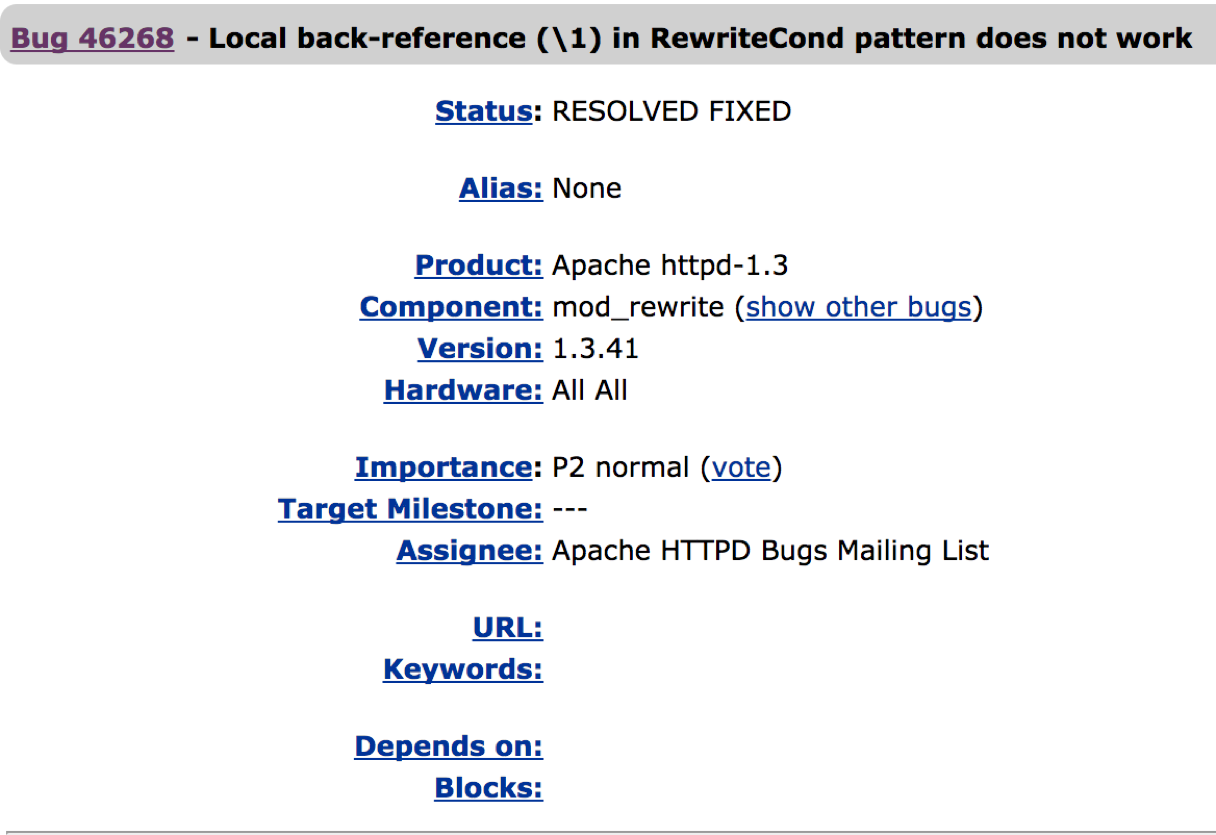
\includegraphics[width=0.8\textwidth]{parikshan/figs/bug-description}
\caption{Metadata description for a Apache semantic bug}	
\label{fig:semanticbugdesc}
\end{center}
\end{figure}

The second part of the bug report (see figure~\ref{fig:semanticcomments}) has a bug description and comment section. Here is the initial description by the user who observed the bug, and potentially ways to recreate the error and the symptoms of the bug. In this example the user explains that he had difficulty in making the regex library to work, in later comments it was explained that this was indeed a bug in the packaging and a different library should have been used and was fixed in later versions. We have primarily manually looked into these bug descriptions to categorize whether this is a semantic, concurrency, performance, or resource leak bug. For cases where this information was not clear or properly explained we have skipped the bug entirely. 

\begin{figure}[!h]
\begin{center}
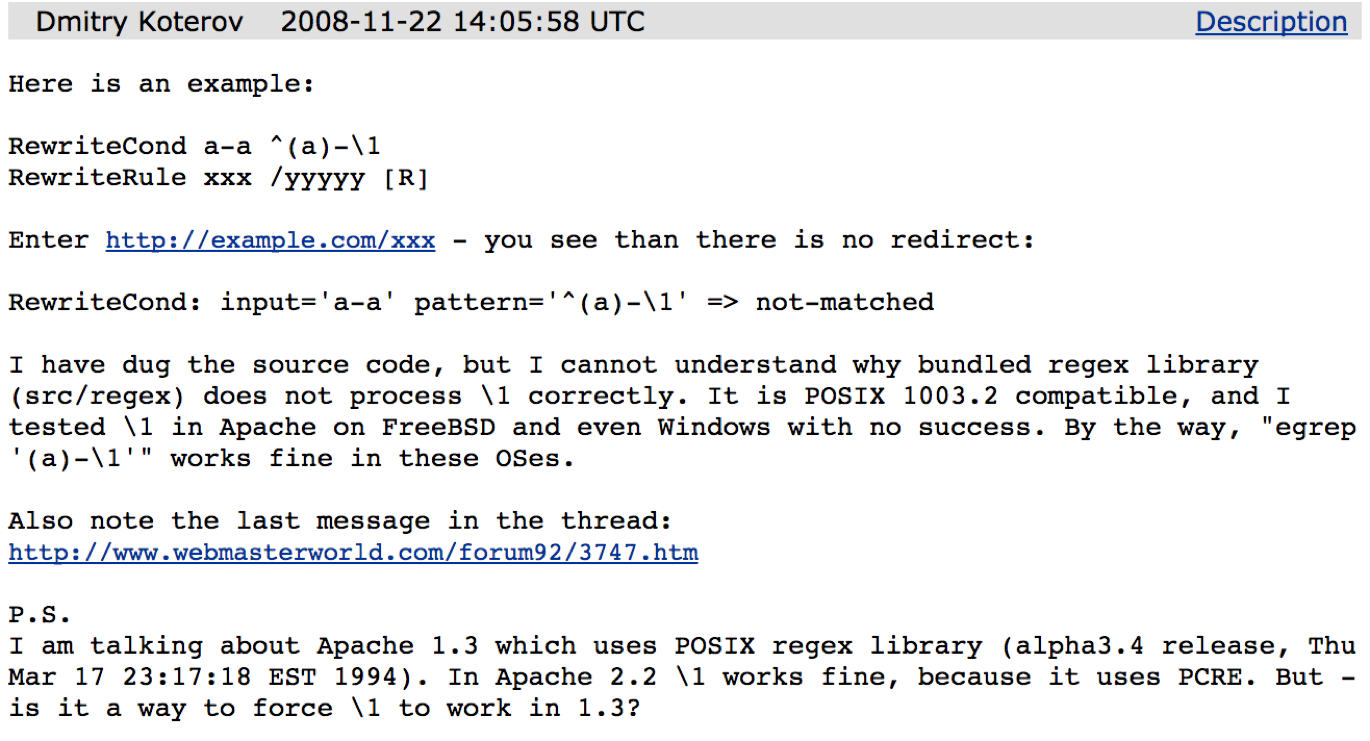
\includegraphics[width=0.8\textwidth]{parikshan/figs/comments}
\caption{Description for a Apache semantic bug based on user report and comments}	
\label{fig:semanticcomments}
\end{center}
\end{figure}

As another example, next we discuss a performance bug in mysql. Figure~\ref{fig:mysqlPerfMeta} shows the meta data information in the bug report. This gives the title of the bug, when the report was submitted, name of the reporter, severity, status and version of MySQL that this bug impacts. As can be seen from the meta-data itself, the severity is S5(Performance). Which itself indicates that the reporter believes this to be a performance bug (please note not all performance bugs are labelled so in the meta-data itself). 
Based on the subject it seems like there is a slow down related to memcached requests.  

\begin{figure}[!h]
	\begin{center}
		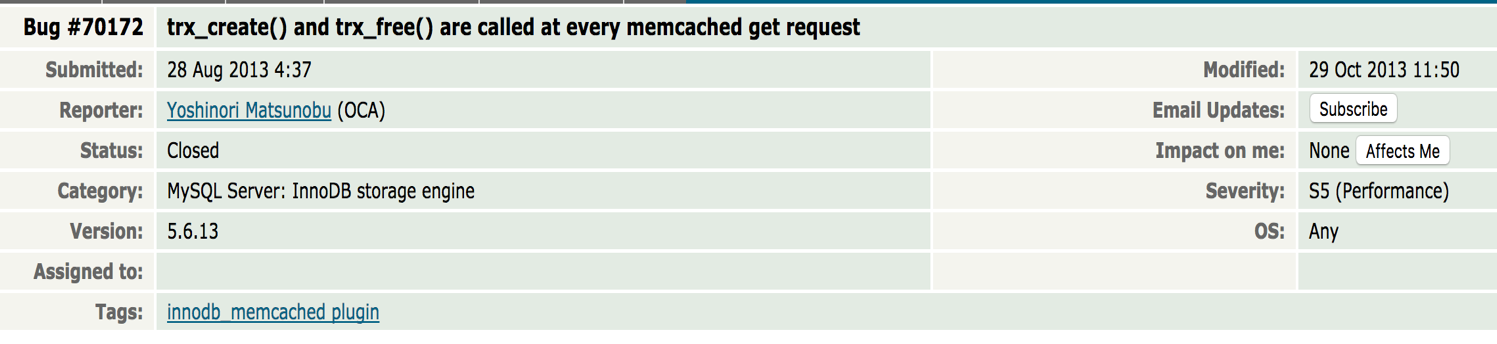
\includegraphics[width=0.8\textwidth]{parikshan/figs/mysqlmeta}
		\caption{Metadata for a performance bug in MySQL}
		\label{fig:mysqlPerfMeta}
	\end{center}
\end{figure}

However, a more detailed explanation of the bug is provided in the bug description section (see figure~\ref{fig:perfcomments}) where the reporter describes the symptoms, and gives a step-by-step process on how to repeat the bug, along with a suggested fix. The bug is caused by repeating create and free calls for each request, which is expensive. Since mysql clients share transaction objects across multiple queries, the reporter believes this should be supported in InnoDB -memcached plugin as well. A comparison between memchached-get vs select shows a bad performance overall from memcached. In the follow up comments it was shown that the request was accepted and the performance bug was fixed for this plugin. 

\begin{figure}
	\begin{center}
		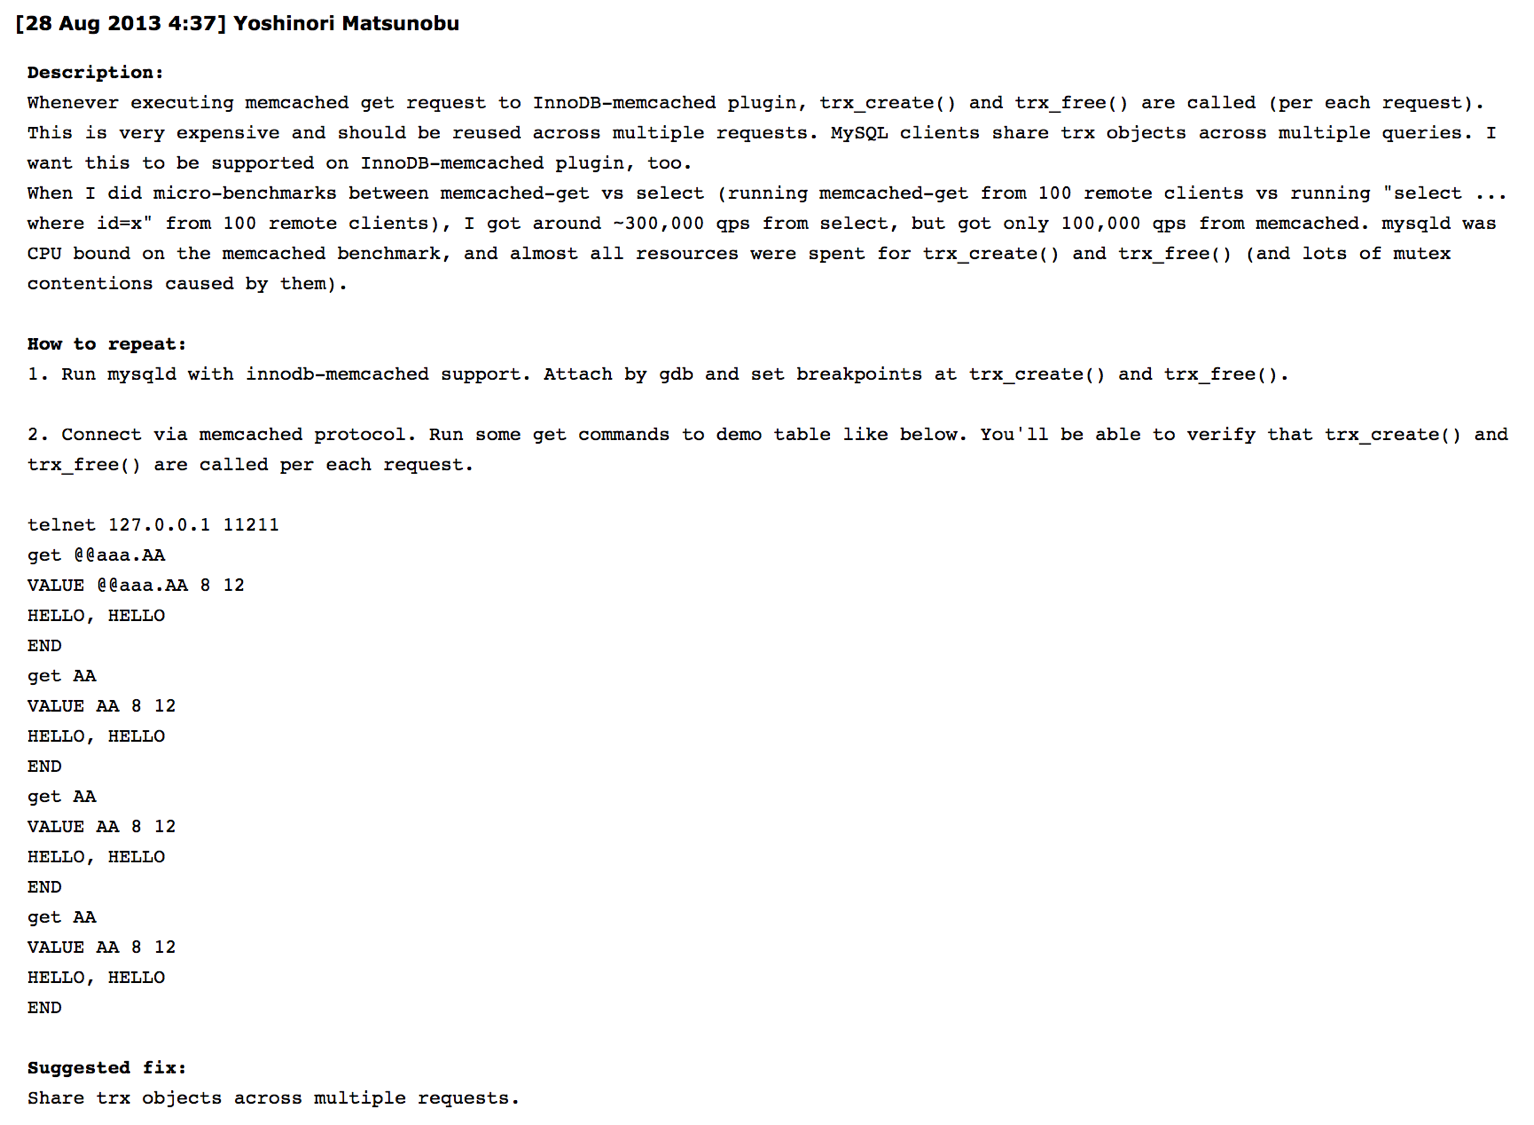
\includegraphics[width=0.8\textwidth]{parikshan/figs/performancedesc}
		\caption{Description for a performance bug}
		\label{fig:perfcomments}
	\end{center}
\end{figure}
%We first searched for bugs which were tagged as ``fixed'' by developers and took a snapshot of them.

As can be seen in the previous bug, it is possible to think of this bug as a feature request since the system is actually working. This is a subjective analysis and really depends on how you want to look at your bug classification. For our bug classification, we have classified performance improvements as performance bugs (as is reported in bugzilla), and semantic changes where a new feature is being suggested as a feature request instead of a semantic bug. All such feature requests have been filtered out and are not considered in this study.


In apache approximately, 38\% of bugs were skipped, and about 14\% could not be categorized. Around 8\% were feature requests, and another 8\% were bugs that actually required documentation updates. Approximately 7\% were related to build issues. In MySQL we selected 102 bugs from 450 bug cases about 60\% of those which were discarded were not focused on the main component, and we took a random selection of bugs from the rest. In MySQL we found two new categories related to fault tolerance and replication (2\% each).


One of the core-insights provided by this survey was that amongst the bugs falling into our 4 major categories most bugs (93\%) triggered in production systems are deterministic in nature (everything but concurrency bugs), among which the most common ones are semantic bugs (80\%).
This is understandable, as they usually happen because of unexpected scenarios or edge cases, that were not thought of during testing.
Recreation of these bugs depend only on the state of the machine, the running environment (other components connected when this bug was triggered), and network input requests, which trigger the bug scenario.
\parikshan is a useful testing tool for testing these deterministic bugs in an exact clone of the production state, with replicated network input. 
The execution can then be traced at a much higher granularity than what would be allowed in production containers, to find the root cause of the bug. 

On the other hand, concurrency errors, which are non-deterministic in nature make up for less than 7\% of the production bugs.
Owing to non-determinism, it is possible that the same execution is not triggered. However concurrent points can still be monitored and a post-facto search of different executions can be done to find the bug~\cite{dpor,systematicDPORconcurrency} to capture these non-deterministic errors. This process is further described in the section on staged record and replay (see section~\ref{sec:activeStagedRecordReplay}).  \\ \\



